% !TEX program = xelatex

\documentclass[12pt,a4paper]{article}

\usepackage{amsthm,amsfonts,amssymb,bm}
\usepackage[fleqn]{amsmath}
\addtolength{\textheight}{2.0cm}
\addtolength{\voffset}{-2cm}
\addtolength{\hoffset}{-1.5cm}
\addtolength{\textwidth}{4.0cm}

%\allowdisplaybreaks

%\usepackage{subeqnarray}
\usepackage{mathrsfs}
%\usepackage{color}
%\usepackage{url}
%\usepackage{ulem}
\usepackage{indentfirst}
%\usepackage{textcomp}
%\usepackage{graphics}
%\usepackage{graphicx}
%\usepackage[hang,small,bf]{caption}
%\setlength{\captionmargin}{50pt}



%%Here is the configuration for chinese. 
%\usepackage[cm-default]{fontspec}
%\usepackage{xunicode}
%\usepackage{xltxtra}
%\setmainfont{AR PL UKai CN}
%\setsansfont[BoldFont=SimHei]{KaiTi_GB2312}
%\setmonofont{NSimSun}

%\XeTeXlinebreaklocale "zh"
%\XeTeXlinebreakskip = 0pt plus 1pt


%\usepackage{tikz}
%\usetikzlibrary{mindmap,trees}
\usepackage{graphicx}
%\usepackage[hang,small,bf]{caption}
%\setlength{\captionmargin}{50pt}

\graphicspath{{Figures/}}

\begin{document}
\title{Power Spectrum of f(R) Gravity Models}
%\author{MA Lei}
%\maketitle

\newcommand{\dd}{\mathrm d}
\newcommand{\HH}{\mathcal H}
\newcommand{\CN}{{\it Cosmologia Notebook}}
\newenvironment{eqnset}
{\begin{equation}\left \bracevert \begin{array}{l}}
{\end{array} \right. \end{equation}}

\newenvironment{eqn}
{\begin{equation}\left \bracevert \begin{array}{l}}
{\end{array} \right. \end{equation}}


\newpage    %It is weird that this command solve the problem that the figure goes between the double line and the text.
\hrule\vspace{1pt}\hrule
\begin{center}
\mbox{{\bf Power Spectra of f(R) Models}} \\
\vspace{0.5em}
\mbox{{}}
\end{center}
\hrule

\setcounter{section}{1}

\subsection{Conventions}
\begin{itemize}
\item
$'=\frac{\mathrm d}{\mathrm d a}$
\item
Lagrange density of gravity
\begin{equation}
\mathcal L=R+f(R)
\end{equation}

\item
$f_R\equiv \frac{\mathrm d f}{\mathrm d R}$.
\item
$f_{RR}\equiv \frac{\mathrm d^2 f}{\mathrm d R^2}$.

\item
$\Omega_{i0}$ is the current fraction density of i component.
\item
$\Omega_i$ is the fraction density of i component at time $a$, i.e., $\Omega_i\equiv \Omega_i(a)$.
\item
$\Omega$ is the total density at time $a$, i.e., $\Omega\equiv \Omega(a)$.

\item
Dimension
\begin{enumerate}
\item
$[H]\sim \mathrm{Mpc^{-1}}$
\item
$[R] \sim \mathrm{Mpc^{-2}}$
\item
$[f(R)]\sim [R] \sim \mathrm{Mpc^{-2}}$

\end{enumerate}

\end{itemize}






%%%%List the models and related
\subsection{Models}

\begin{itemize}
\item
Hu\&Sawicki Model
\begin{equation}
f_{HS}=-m^2\frac{C_1 (\frac{R}{m^2})^n}{C_2 (\frac{R}{m^2})^n + 1}\label{HSMod}
\end{equation}
Its series expansion at $m^2/R\sim 0$ is \footnote{From LCDM model, this quantity is much smaller than 1 through out the history. Three orders are kept because its second derivative of $R$ will be used.}
\begin{equation}
f_{HS}\approx -\frac{C_1}{C_2}_1m^2+\frac{C_1}{C_2^2}m^2(\frac{m^2}{R})^n-\frac{C_1}{C_2^3}m^2 (\frac{m^2}{R})^{2n}+\frac{C_1}{C_2^4}m^2(\frac{m^2}{R})^{3n}
\end{equation}
\item
Starobinsky Model
\begin{equation}
f_{S}=\lambda R_s[(1+\frac{R^2}{R_s})^{-n}-1] \label{SbMod}
\end{equation}
Its series expansion at $R_s^2/R^2\sim 0$ is 
\begin{eqnarray}
f_S &\approx& -\lambda R_S+\lambda R_S (\frac{R_S^2}{R^2})^n-\lambda R_S\cdot n (\frac{R_S^2}{R^2})^{n+1} +\lambda R_S\cdot\frac12 (n+n^2)(\frac{R_S^2}{R^2})^{n+2}\\
&&-\lambda R_S \cdot \frac16(2n+3n^2+n^3)(\frac{R_S^2}{R^2})^{n+3}
\end{eqnarray}
\item
Tsujikawa Model
\begin{equation}
f_T=-\mu R_T \tanh(\frac{R}{R_T})
\end{equation}
Its approximation at $R_T/R<<1$ is
\begin{equation}
f_T\approx -\mu R_T +2\mu R_T e^{-2\frac{R}{R_T}}-2\mu R_T e^{-4\frac{R}{R_T}}+2\mu R_T e^{-6\frac{R}{R_T}}-2\mu R_T e^{-8\frac{R}{R_T}}+2\mu R_T e^{-10\frac{R}{R_T}}
\end{equation}
\item
Exponential Gravity Model
\begin{equation}
f_E=-\beta R_E(1-e^{-R/R_E}) \label{TkMod}
\end{equation}
\end{itemize}


\subsection{Hu\&Sawicki Model}

\subsubsection{Parameters and more}
\begin{itemize}
\item[.]
$n=1$
\item[.]
$d_1=6\frac{\Omega_{x0}}{\Omega_{m0}}$
\item[.]
$d_2=-f_{R0}\left( \frac{12}{\Omega_{m0}}-9 \right)^2$
%\item[.]
%$C_1(n)=-\frac{36(\Omega_{x0}/\Omega_{m0})^2}{(12/\Omega_{m0}-9)^{n+1}}\frac{n}{f_{R0}}$
%\item[.]
%$C_2(n)=-\frac{6\Omega_{x0}/\Omega_{m0}}{(12\Omega_{m0}-9)^{n+1}}\frac{n}{f_{R0}}$
\item[.]
$\Omega=\Omega_{m0}a^{-3}+\Omega_{r0}a^{-4}$
\end{itemize}

\subsubsection{Background}


Hubble function is just an rearrangement of Friedmann equationk, which is
\begin{equation}
H=\sqrt{\frac{H_0^2\Omega+\frac{1}{6}(f_R\cdot R-f)}{1+f_R+3a f_{RR}\cdot R'}}\label{Eq-ModHub}
\end{equation}

For Hu\&Sawicki' model, the related terms are
\begin{enumerate}
\item[*]
$R=3H_0^2\Omega+2d_1 m^2$. \qquad\footnote{Wayne Hu and Ignacy Sawicki, Models of $f(R)$ cosmic acceleration that evade solar system tests, Phys. Rev. D 76, 064004 (2007).}
\item[*]
$f\approx -\frac{C_1}{C_2}m^2+\frac{C_1}{C_2^2} m^2\frac{m^2}{R^2}-\frac{C_1}{C_2^3}m^2(\frac{m^2}{R})^2+\frac{C_1}{C_2^4}(\frac{m^2}{R})^3$
\item[*]
$f_R\approx -\frac{C_1}{C_2^2}(\frac{m^2}{R})^2+2\frac{C_1}{C_2^3}(\frac{m^2}{R})^3$
\item[*]
$f_{RR}\approx 2\frac{C_1}{C_2^2}\frac{m^4}{R}$
\end{enumerate}

Put them into Eq (\ref{Eq-ModHub}),and drop high order terms,
\begin{equation}
H=H_0\sqrt{\frac{\Omega+\frac16 d_1 \Omega_{m0}-\frac13 d_2 \Omega_{m0}\frac{1}{\hat R}a^{-3}}{1-d_2\frac{\Omega_{m0}^2}{\hat R^2}-27\times 2 d_2 \frac{\Omega_{m0}^3}{\hat R^3}a^{-3}}},
\end{equation}
where $d_1\equiv \frac{C_1}{C_2}$, $d2\equiv \frac{C_1}{C_2^2}$, $\Omega= \Omega_{m0}a^{-3}+\Omega_{r0}a^{-4}$.



\subsubsection{Perturbation Theory}

Perturbation equation in Newtonian gauge, matter domination era and later
\begin{equation}
\delta_m'' + \left(\frac{H'}{H}+\frac{3}{a}\right)\delta_m'-\frac32 \bar \chi_{eff} \frac{H_0^2}{aH^2}\Omega_m\delta_m=0 \label{Eq-HSModPer},
\end{equation}
where $\bar \chi_{eff}\equiv\frac{\chi_{eff}}{\chi}=\frac{1}{f_R+1}\frac{4+(\frac{f_R+1}{f_{RR}-R})\frac{a^2}{k^2}}{3[1+\frac13(\frac{f_R+1}{R_{RR}}-R\frac{a^2}{k^2})]}$, $\chi_{eff}^2\equiv 8\pi G_{eff}$ is corresponds to $\chi^2\equiv8\pi G$  in LCDM.

A numerical calculation shows $\bar\chi_{eff}$ doesn't change the solutions of the perturbation. I have checked both large $k$ and small $k$ at about $a\sim 10$, the result doesn't change at a four digit precision.
Besides, I plotted out $\bar\chi_{eff}$ (figure \ref{Fig-HSMod-chi}) and it only starts change slightly at about $a=0.2$. So I drop this $\bar\chi_{eff}$ term in the following numerical calculation.



\subsubsection{Results}

\begin{figure}[!htpb]
\centering
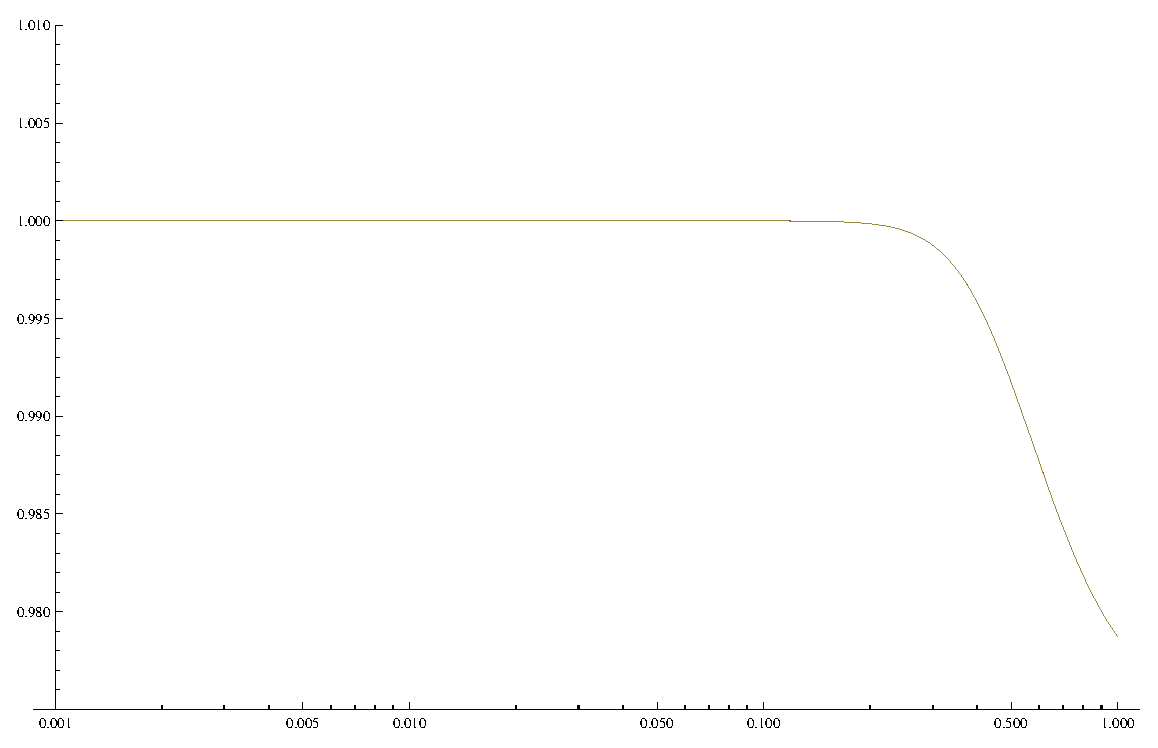
\includegraphics[width=300pt]{HSMod-chi.eps}
\caption{$\bar\chi_{eff}$ of Hu\&Sawicki model.}\label{Fig-HSMod-chi}
\end{figure}



Figure \ref{Fig-HSMod-Bub} shows the Hubble function.

\begin{figure}[!htpb]
\centering
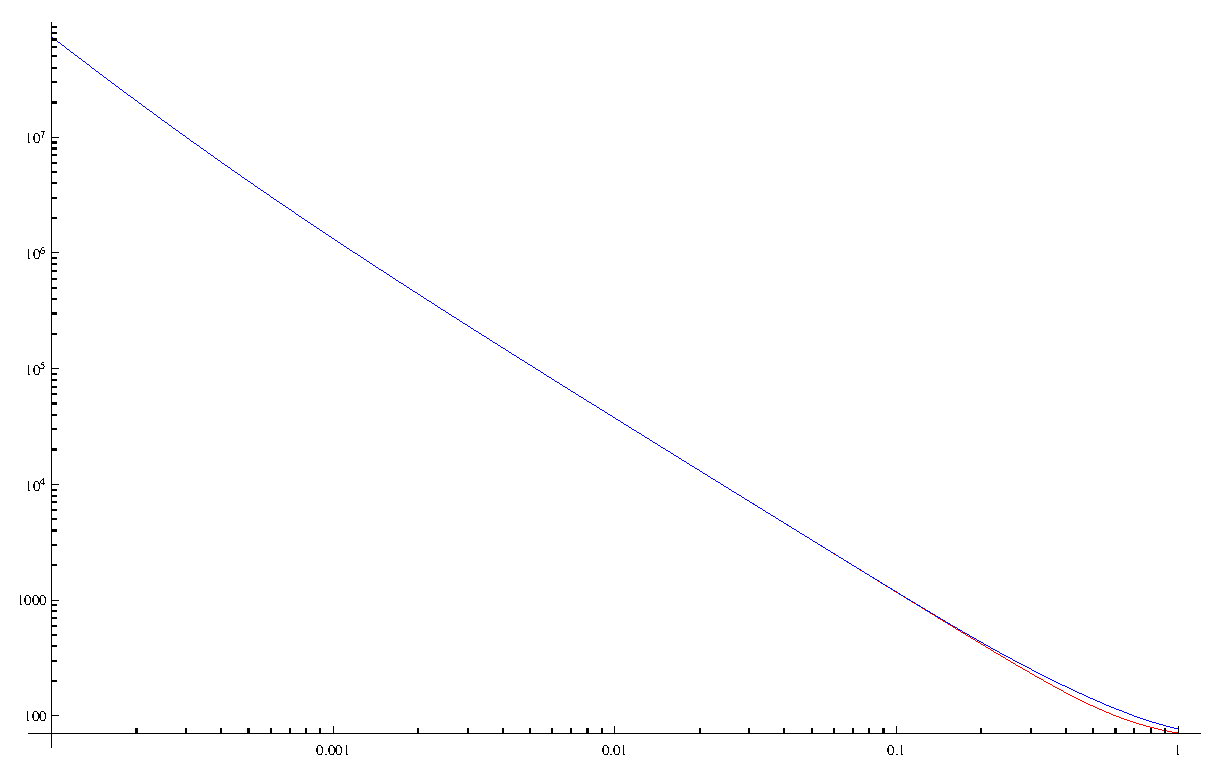
\includegraphics[width=300pt]{HSMod-Hub.eps}
\caption{Hubble function of Hu\&Sawicki model and LCDM. Upper line (blue) is the Hu\&Sawicki model. Lower line (red) is for LCDM.}\label{Fig-HSMod-Bub}
\end{figure}


Figure \ref{Fig-HSMod-EoSEff} is the effective equation of state of Hu\&Sawicki model.

\begin{figure}[!htpb]
\centering
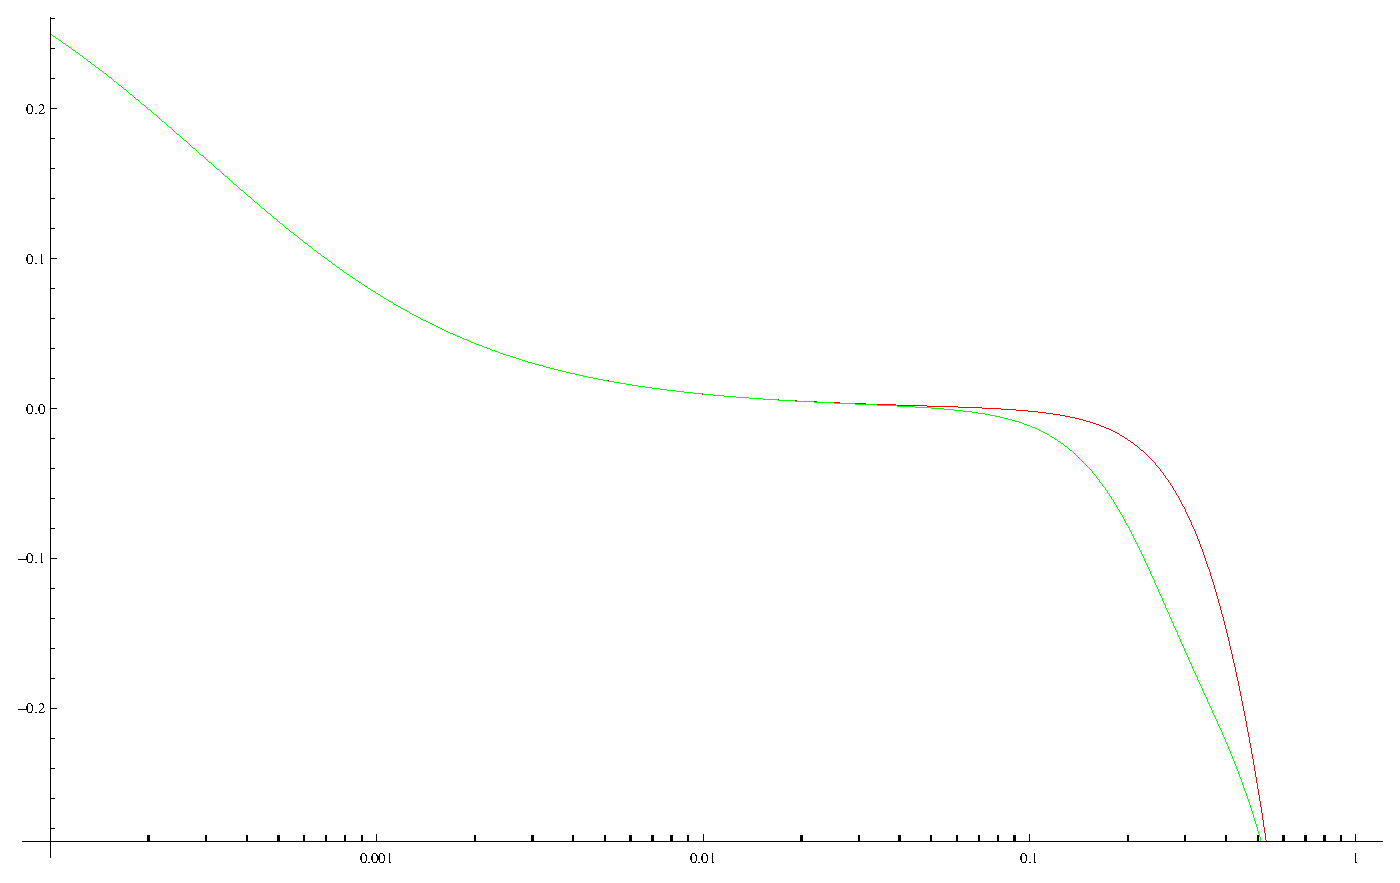
\includegraphics[width=300pt]{HSMod-EoSEff.eps}
\caption{Effective EoS of Hu\&Sawicki model. Red line is LCDM model while green line is Hu\&Sawicki model.}\label{Fig-HSMod-EoSEff}
\end{figure}


Figure \ref{Fig-HSMod-Growth} is the growth function of Hu\&Sawicki model. (It is a pity that this figure does not completely show the growth function.)

\begin{figure}[!htpb]
\centering
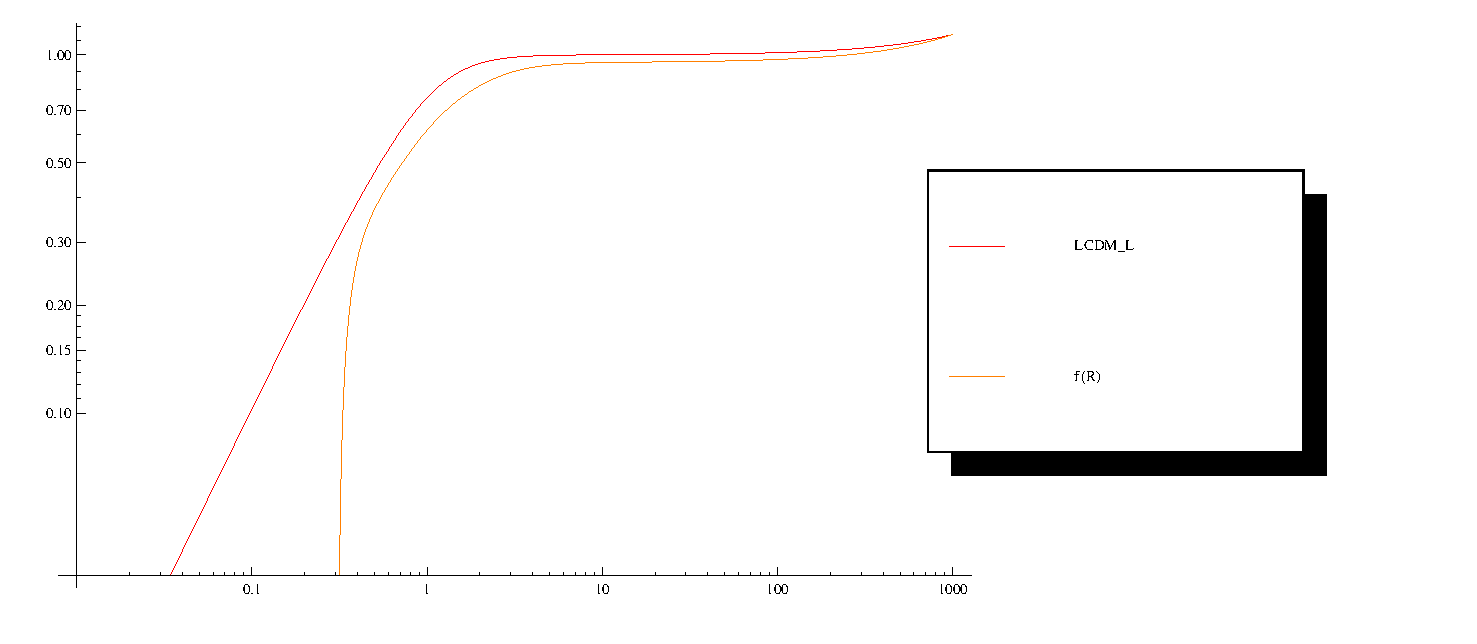
\includegraphics[width=300pt]{HSMod-Growth.eps}
\caption{Growth function of Hu\&Sawicki model.}\label{Fig-HSMod-Growth}
\end{figure}


Figure \ref{Fig-HSMod-QFac} is $Q=\frac{\text{Power of Hu\&Sawicki model}}{\text{Power of LCDM model}}$ factor. (I do not have the power spectra of LCDM in Newtonian gauge, so this is the furthest I can go.)

\begin{figure}[!htpb]
\centering
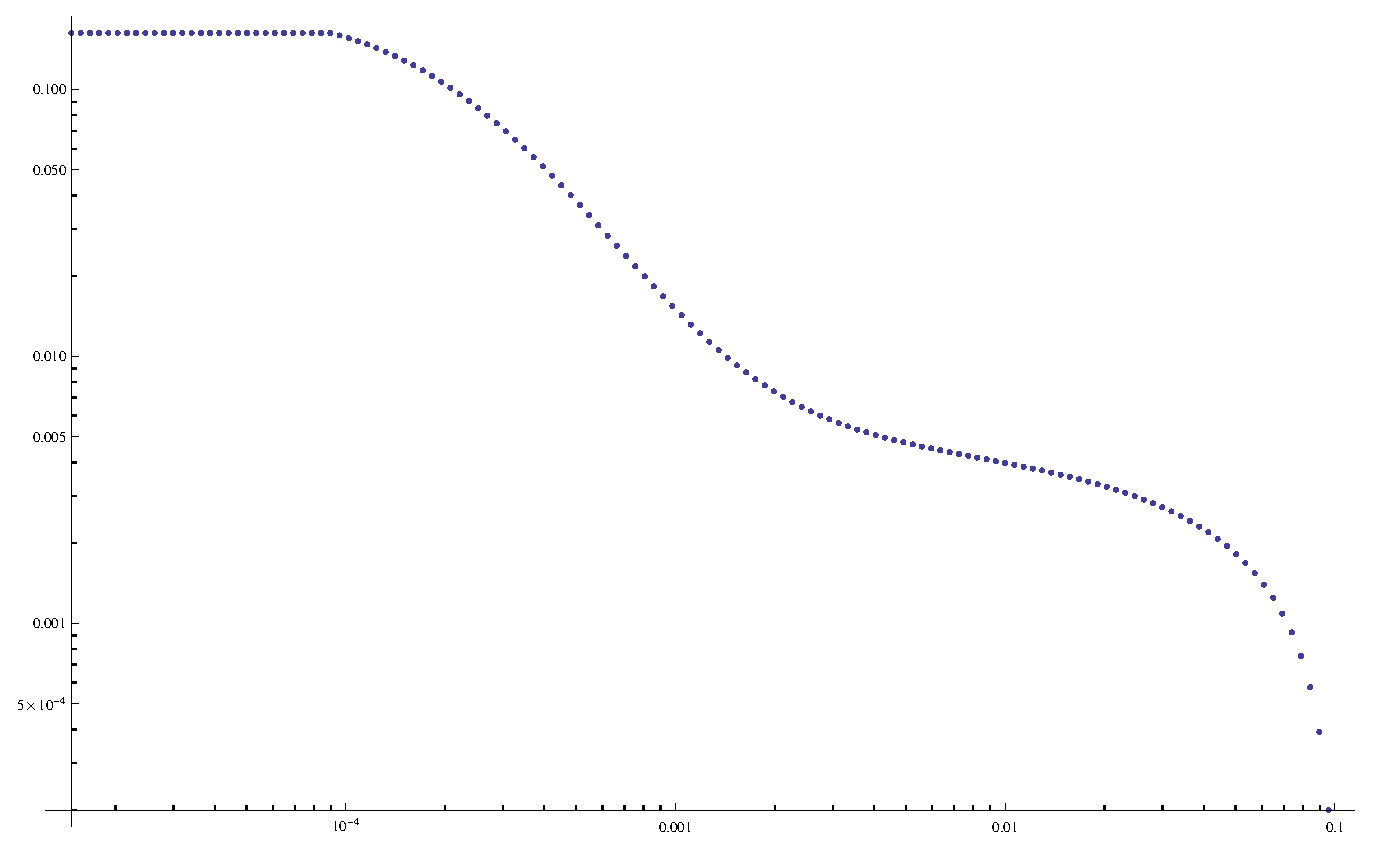
\includegraphics[width=300pt]{HSMod-QFac.eps}
\caption{$Q=\frac{\text{Power of Hu\&Sawicki model}}{\text{Power of LCDM model}}$.}\label{Fig-HSMod-QFac}
\end{figure}





\subsection{Starobinsky Model}

\subsubsection{Parameters}
\begin{itemize}
\item[.]
$n=1$
\item[.]
$\lambda=6\frac{\Omega_{x0}}{\Omega_{m0}}$
\item[.]
$R_S=H_0^2\Omega_{m0}$
\end{itemize}

\subsubsection{Background}

\begin{enumerate}
\item[*]
$f=-\lambda\frac{R_S}{c^2}+\lambda \frac{R_S}{c^2}\frac{R_S^2}{R^2}-\lambda \frac{R_S}{c^2}(\frac{R_S^2}{R^2})^2$
\item[*]
$f_R=-2\lambda \frac{R_S^3}{R^3}+4\lambda \frac{R_S^5}{R^5}$
\item[*]
$f_{RR}=6\lambda \frac{R_S^3}{R^4}c^2$
\end{enumerate}

A similar method (using Eq (\ref{Eq-ModHub})) shows the background of Starobinsky's model. (Since the  equation is a bit complicated, I won't write it here. It is in a mathematica notebook.)

\subsubsection{Perturbations}

Similar to Hu\&Sawicki's model, that $\bar\chi_{eff}$ can be substituted by 1. The fact is this model adds much less corrections to LCDM than Hu\&Sawicki's.

\subsubsection{Results}

Figure \ref{Fig-SBMod-chi} is $\bar\chi_{eff}$.

\begin{figure}[!htpb]
\centering
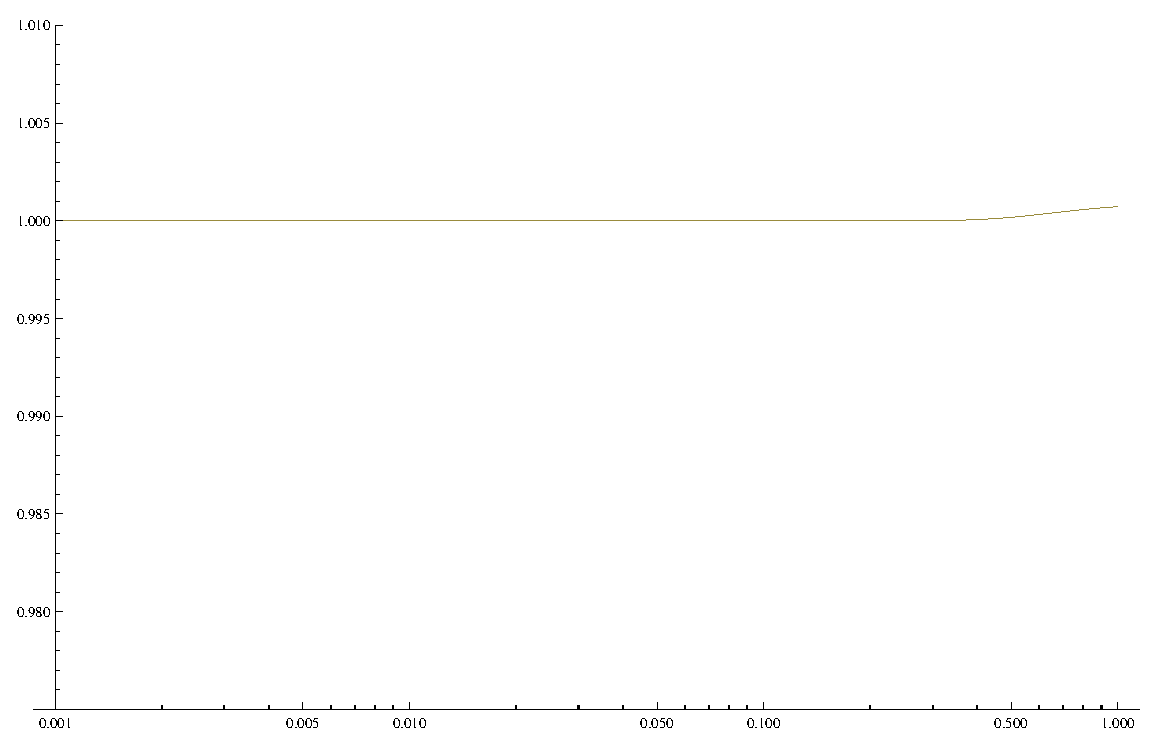
\includegraphics[width=300pt]{SBMod-chi.eps}
\caption{$\bar\chi_{eff}$ of Starobinsky' model.}\label{Fig-SBMod-chi}
\end{figure}


Figure \ref{Fig-SBMod-Hub} is the Hubble function of Starobinsky' model. The two lines are the same. (Not really the same, the deviations are too small to be shown.)
\begin{figure}[!htpb]
\centering
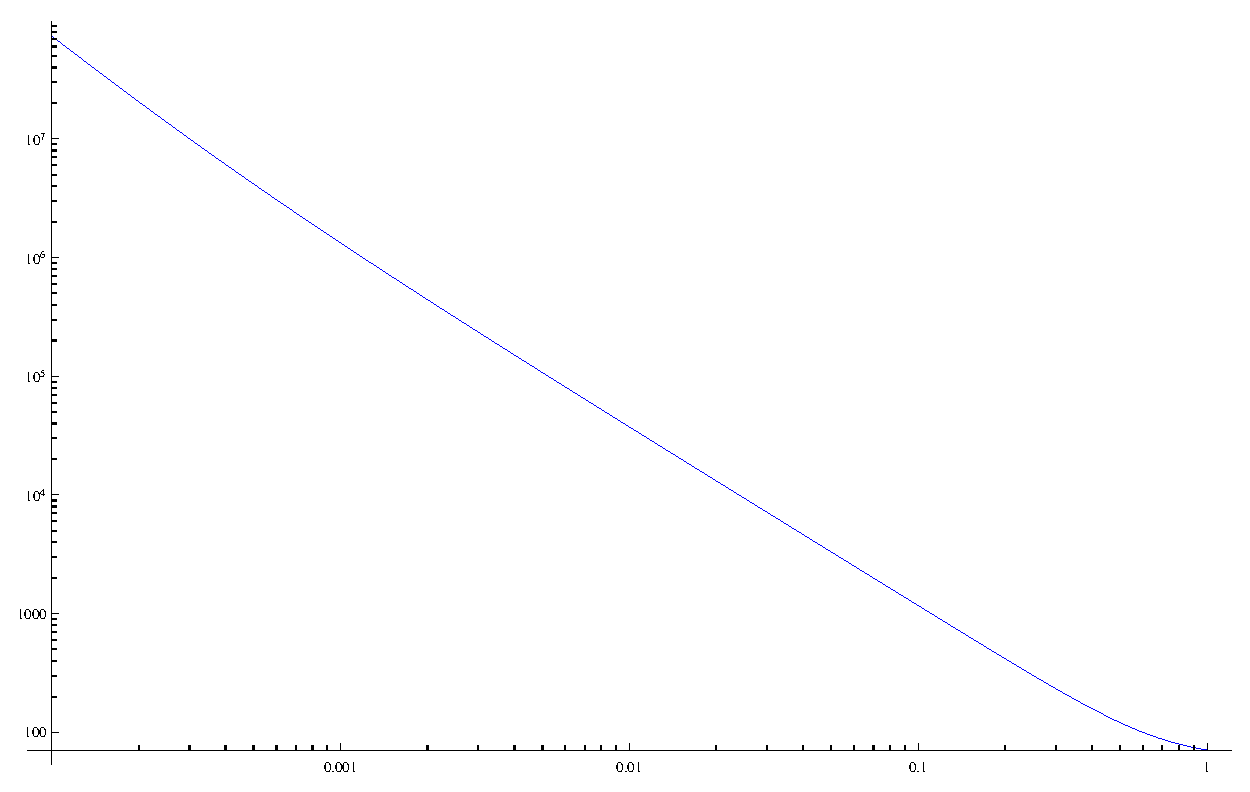
\includegraphics[width=300pt]{SBMod-Hub.eps}
\caption{Hubble function of Starobinsky's model and that of LCDM. They are completely the same in this figure.}\label{Fig-SBMod-Hub}
\end{figure}



Figure \ref{Fig-SBMod-EoSEff} is the effective equation of state.
\begin{figure}[!htpb]
\centering
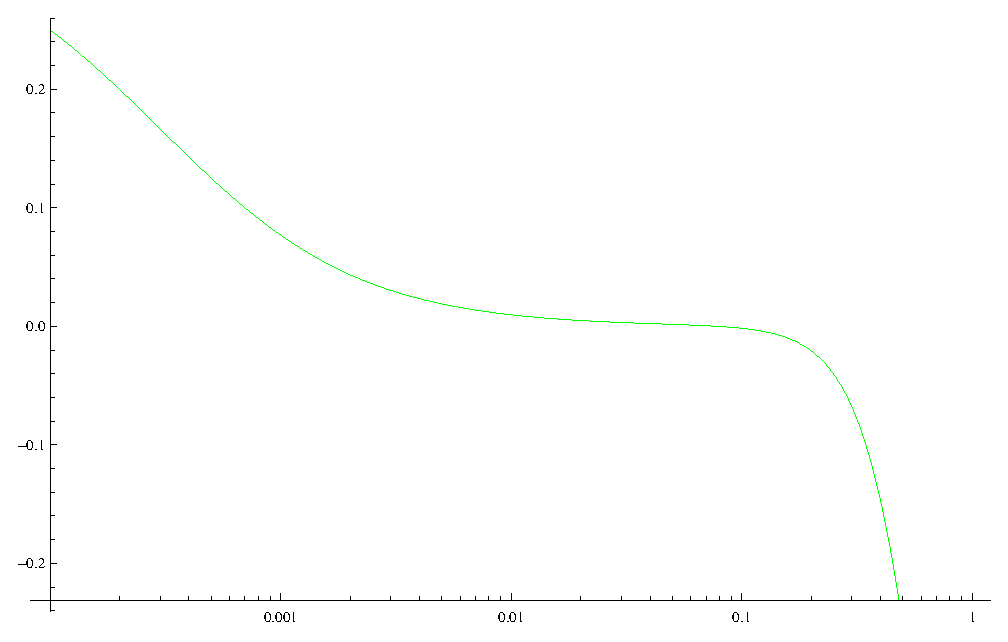
\includegraphics[width=300pt]{SBMod-EoSEff.eps}
\caption{Effective equation of state are the same too.}\label{Fig-SBMod-EoSEff}
\end{figure}

Figure \ref{Fig-SBMod-Growth} is the growth function of Starobinsky's model.
\begin{figure}[!htpb]
\centering
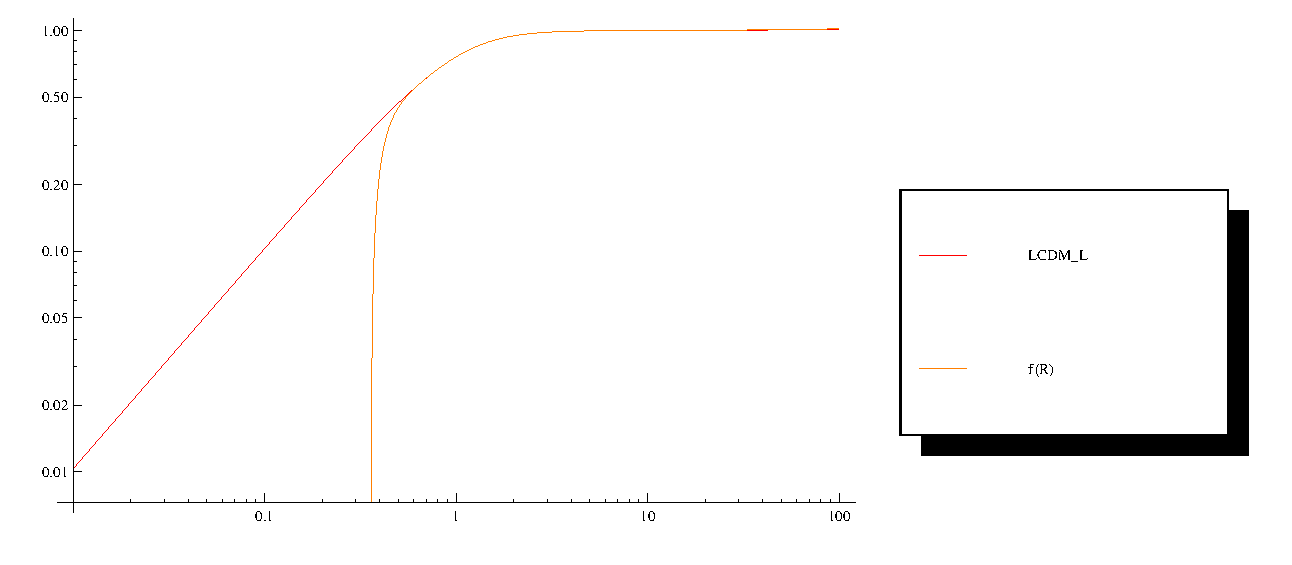
\includegraphics[width=300pt]{SBMod-Growth.eps}
\caption{Growth function of Starobinsky's model.}\label{Fig-SBMod-Growth}
\end{figure}



Figure \ref{Fig-SBMod-QFac} is $Q=\frac{\text{Power of Hu\&Sawicki model}}{\text{Power of LCDM model}}$.
\begin{figure}[!htpb]
\centering
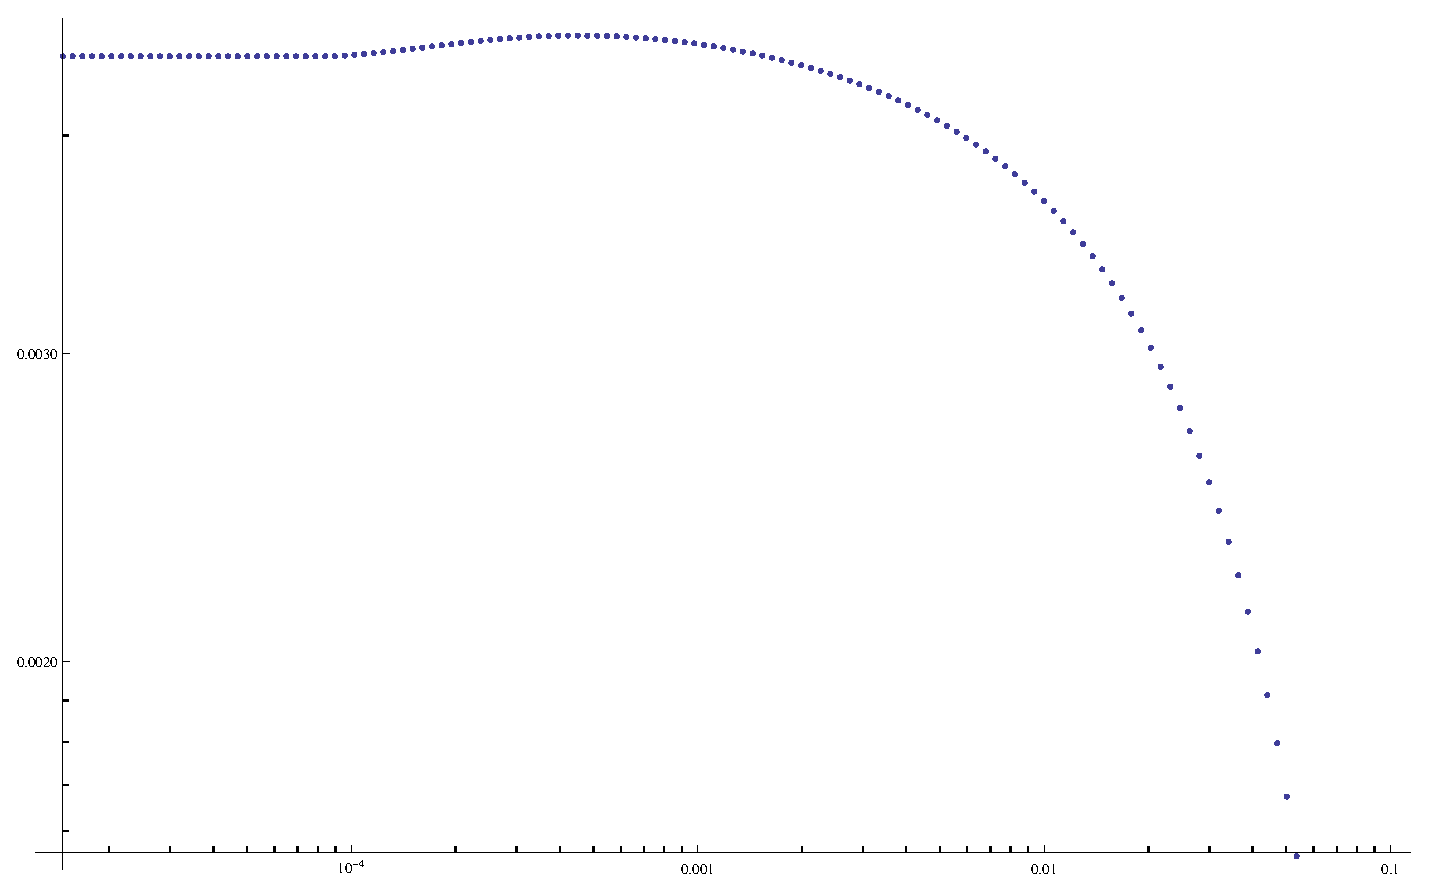
\includegraphics[width=300pt]{SBMod-QFac.eps}
\caption{$Q=\frac{\text{Power of Hu\&Sawicki model}}{\text{Power of LCDM model}}$ of Starobinsky's model.}\label{Fig-SBMod-QFac}
\end{figure}





\end{document}